\chapter{Региональный потенциал оптической модели с учетом колебательных и вращательных возбуждений для актинидов}

\section{Методика поиска параметров оптического потенциала}

\begin{itemize}
    \item Выбор схем связи для рассматриваемых ядер
    \item $\chi^2$
    \item Расчет параметров оптического потенциала на основе экспериментальных 
данных для 238U и 232Th
    \item Определение деформаций остальных ядер для описания имеющихся 
экспериментальных данных
\end{itemize}

\section{Расчет оптических сечений для рассматриваемых ядер с помощью полученного
единого потенциала}

\section{Сравнение результатов расчета с другими оптическими моделями}

\section{Анализ изменений в сечениях, возникающих из-за рассмотрения мягкости ядер и связи уровней из нескольких полос}

\begin{figure}[ht!]
\begin{center}
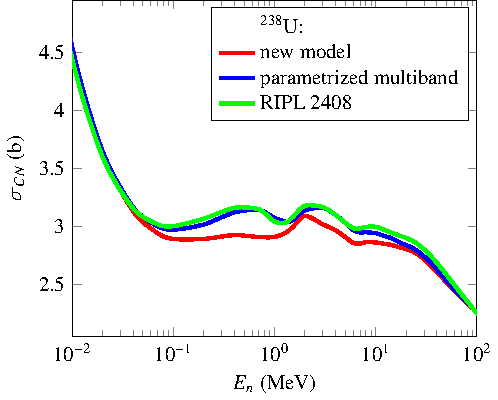
\includegraphics[width=0.7\textwidth]{images/fig1a.pdf}\\
\caption{Подпись к рисунку. Дополнительная информация}
\label{app:fig}
\end{center}
\end{figure}

дйфдфд \cite{myarticle,myrussianarticle,myproc,mybook}